\documentclass[12pt]{article}
\usepackage[english]{babel}
\usepackage[utf8]{inputenc}
\usepackage{graphicx}
\usepackage{amsmath,amssymb}
\usepackage{hyperref}
\usepackage{geometry}
\geometry{a4paper, top=2cm}

\hypersetup{colorlinks=true, urlcolor=blue, linkcolor=blue, citecolor=red} %

\title{Cognitive Robotics Lab Report}
\author{Sean Parker\\
34212-Lab-S-Report}

\begin{document}
\maketitle

\section{Introduction}
The aim of this report is to describe the current problem in computer vision for solving image recognition, which is very important in the area of robotic vision, to describe the current state-of-the-art network architectures and finally to descirbe my approach for solving this problem. This project used the CIFAR-10 dataset which consists of 60000 32x32 colour images, grouped into 10 classes. Although the dataset has low quality images, and for a real-world robot it's visual acuity would be much greater (for example iCub which use 2x Dragonfly2 camera, each with a resolution of 648x488 pixels), solving image recognition on a simple dataset provides a proof of concept for a system that could be upscaled in order to perform image recognition on higher resolution images.

Firstly, the network architecture was chosen before evaluation of the network with a selection of hyperparameters. In order to find a good architecture, I researched the current state of the art (see Section \ref{sec:soa}) in order to find the top class performance. Using a very deep CNN architecture, one can achieve an error rate of only 1.0\%\cite{huang2018gpipe}, however this architecture has over 500-million parameters which is far too large for the available computer power for this project, additionally the model in the paper is trained using distributed GPUs and Google Colab only supports single GPU training.

Therefore, I looked for simplier network architectures that still achieved good results on the CIFAR dataset. After some research in modern techniques to improve training networks, I decided to include layers using Batch Normalisation and Dropout layers which have been shown to improve the accuracy of networks\cite{dropout, batch-norm}.

Lastly, in terms of hyperparameter choice, there were some main hyperparameters that had to be refined for the network topology. The main hyperparameters that had to be defined were the learning rate of the optimiser, and weight decay for L2 regularization. Additionally, the network topology is a based on blocks of (CONV + ELU + Batch Norm)\footnote{In this case, ``+'' refers to a combination of ideas, rather than the plus operator in mathematics.}. More details of the network architecture can be found in Section \ref{sec:imple}.

\section{State of the art}
\label{sec:soa}
Over the past decades, there has been a ever accelerating improvement with neural networks, convolution neural networks and other architectures that have been developed. Over the past 5-7 years, a renewed focus has been on deep neural networks, trying to overcome the problem of vanishing graidents. In this effort, the networks have been able to ``adapt'' to new experiences much faster and with much greater accuracy. \cite{imagenet, howard2019searching}

Modern networks have millions of parameters and can take days or even weeks to train; with the advances in GPU parallel processing it takes a long time. However, once trained, the models don't require a large amount of processing power, hense, for robotics this can lead to cheaper robots where the designer can instead make investment into better joints/motors. Also, with the advancement of DNN (Deep neural networks), the networks (and therefore the robots) can operate on the raw sensor data, without little or no pre-processing.

Another common network architecture used for robotics is one called \textit{``autoencoders''}. It requires two CNNs, one that acts as the \textit{``encoder''} and the other as the \textit{``decoder''}. The benefit of this architecture is that the network can create a hidden state, and since the designer may not know beforehand the values needed to represent the system, the autoencoder can learn autonomously.

In terms of the current task of computer vision where we aim to classify images into a set of categories. The current state of the art was set in 2018 by Y. Huang et al. with the release of ``GPipe'' which is a technique used for training massive models using pipeline parallelism, achieving an accuracy of 99\% on CIFAR-10.


\section{Implementation}
\label{sec:imple}
After testing different architectures, I found a good middle ground between network complexity, training time, and performace was the following architecture.

Firstly, we expect the input to be a 32x32 input image with three channels (RGB). The network consits of three blocks, each using the same architecture, but with different hyperparameters. The structure of each block is as follows. Convolution of filters with stride 1, L2 regularization (weight decay of $1\times 10^{-4}$), ELU activation, and Batch Normalisation. Next, aonther Convolution layer, ELU activation and Batch Normalisation. Finally, the block finishes with Max pooling (size of 2x2), ELU activation and a dropout layer.

We repeat this structure two more times, before finally flattening the output layer with a single dropout layer which is connected to a fully connected layer with 10 units. These units predict the category in which the image should be classified.

The choice of using ELU activation over ReLU activation was that the ELU activation function (shown below) leads to higher classification accuracies and helps prevent the problem of vanishing graidents in the layers \cite{clevert2015fast}.

\begin{figure}[htbp]
  \centering
  \begin{minipage}{0.4\textwidth}
    \centering
    \begin{equation}
      ELU(x) = \begin{cases} x                 & \text{if}~x > 0    \\
        \alpha ( e^x - 1) & \text{if}~x \leq 0\end{cases}
    \end{equation}
  \end{minipage}\hfill
  \begin{minipage}{0.4\textwidth}
    \centering
    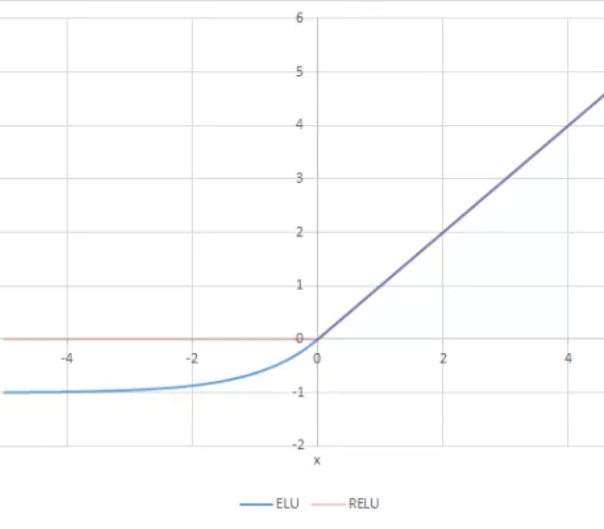
\includegraphics[width=1\textwidth]{results/eluvsrelu.png}
    \caption{ELU vs ReLU activation functions
      \label{fig:eluvsrelu}
    }
  \end{minipage}
\end{figure}
\newpage

Additionally, I also used a learning rate schedule in order to start with a high learning rate at the start of training, and then at specific points during training, the learning rate is reduced in order to perform fine-tuning. The optimiser used for the network was RMSprop with batch sizes of 128. The schedule that I found produced the best results was the following:

\begin{itemize}
  \item Learning rate = 0.001 when epoch $\geq 0$
  \item Learning rate = 0.0005 when epoch $\ge 25$
  \item Learning rate = 0.00025 when epoch $\ge 50$
  \item Learning rate = 0.000075 when epoch $\ge 80$
\end{itemize}

Finally, the training was performed for 100 epochs, I found this was a good balance between training time and performance. Using the learning rate schedule above, around epoch 60, the accuracy reached 83\% at which point the network needed fine tuning in order to reach the final accuracy of 87\%. Using Google Colab and a NVIDIA P100, it took $\approx 20$s per epoch, in total around 30 minutes to train the model completely.

\section{Experiments}
This section will describe the process of finding the optimal hyperparameters for the network in order to get the best performance. My approach to find these was in large part trail and error, documenting each run with the loss and accuracy, both during the training and testing phases. The starting point for the hyperparameter search was that of the papers that introduced some of the techniques used in the report \cite{simonyan2014deep}.

On the other hand, learning rate is the not the only hyperparameter that affects the accuracy of the model. Since I used L2 regularization in the convolutional layers, weight decay is very important. I first started with the weight decay of $5\times 10^{-4}$ \cite{simonyan2014deep}, however, I found, experimentallly, this was too high for this task. I therefore decreased the weight decay until it decreased the models accuracy rather than it increasing. The final value for weight decay was $1\times 10^{-4}$.

As can be seen in Figures \ref{sch1} and \ref{sch3}, by keeping all else the same, just changing the learning rate has a large effect on the overall accuracy of the network. It is important to note that since we use random initalisation of the network, some tests may start closer to a local minima than others. However, the overall effect can still be observed by looking at the results. Too low of a learning rate means the network will struggle to learn the classification, and too high learning rate leads to quickly overfitting the training data and getting stuck in a poor local minimum.

A promising area of hyperparameter exploration is that of Bayesian hyperparameter optimisation which has been shown to lead to better performance over hand tuning of the learning rates \cite{snoek2012practical, bayesian-optim}.

\begin{figure}[htbp]
  \centering
  \begin{minipage}{0.33\textwidth}
    \centering
    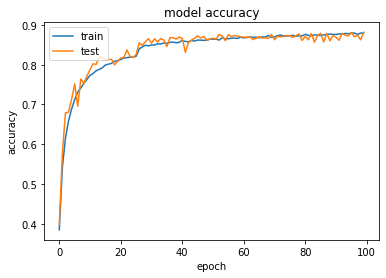
\includegraphics[width=1\textwidth]{results/acc-best.png} % first figure
    \caption{Test Accuracy -- Schedule 1}
    \label{sch1}
  \end{minipage}\hfill
  \begin{minipage}{0.33\textwidth}
    \centering
    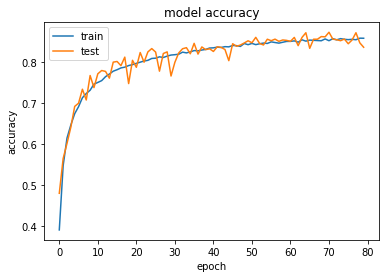
\includegraphics[width=1\textwidth]{results/acc-4.png} % second figure
    \caption{Test Accuracy -- Schedule 2}
  \end{minipage}\hfill
  \begin{minipage}{0.33\textwidth}
    \centering
    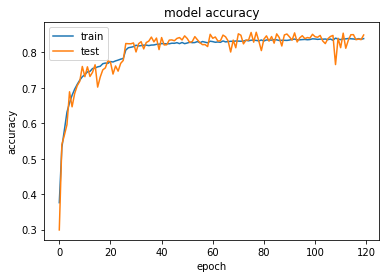
\includegraphics[width=1\textwidth]{results/acc-8.png} % third figure
    \caption{Test Accuracy -- Schedule 3}
    \label{sch3}
  \end{minipage}
\end{figure}

Figure \ref{sch1} shows the best result from the tests, it converges more quickly and the learning is much more stable then compared to the model in Schedule 3. In Figure \ref{sch1} we can see a sharp jump in the accuracy of the model, this is due to the learning rate schedule which dynamically changes learning rate at predefined points during training; therefore, we know that the schedule we defined is helping to perform fine tuning. Figure \ref{sch1} achieves the best performance of 86.9\%.

Overall, many different models were trained and tested fully, each with a slightly different architecture in order to find a suitable model. Table 1 shows an overview of the evolution of the network showing the size of model (number of parameters) and the accuracy the model achieved, not all of the tests are shown, but the trend is clear that the model improved, both in overall accuracy and preventing overfitting of the model.


\begin{table}[htbp]
  \centering
  \begin{tabular}{|c|c|c|c|c|}
    \hline
    Test   & \multicolumn{1}{l|}{Epochs} & \multicolumn{1}{l|}{Training accuracy} & \multicolumn{1}{l|}{Test accuracy} & \multicolumn{1}{l|}{\# of parameters} \\ \hline
    Run 1  & 40                          & 91.3\%                                 & 75.3\%                             & 1,676,842                             \\ \hline
    Run 4  & 80                          & 85.8\%                                 & 82.3\%                             & 1,676,842                             \\ \hline
    Run 10 & 120                         & 86.7\%                                 & 84.4\%                             & 308,394                               \\ \hline
    Best   & 100                         & 88.0\%                                 & 86.9\%                             & 308,394                               \\ \hline
  \end{tabular}
\end{table}

\section{Conclusion}
In conclusion, the challenges posed by computer vision for robotics are difficult to solve, however, with large enough models, powerful hardware to train and enough training data, models can be trained that exceed human performance in these tasks. Although individuals may not currently be able to achieve levels of performace like we described in Section 2, one can produce good models with $>$85\% accuracy in a short amount of time with a small amount of data augmentation. This is only going to improve over time, the training techniques become more refined, and importantly, hardware gets faster and cheaper. This has important implications for robotics, as these high performing models can trained on powerful hardware but executed on mobile platforms such as robots.

In terms of future work, there are many different paths one could research. As discussed, distributed training is an important step in improving training efficiency of these models but also investigating other techniques such as auto-encoders could lead to state of the art performance in these tasks.

\nocite{*}

\bibliographystyle{unsrt}
\bibliography{refs}

\end{document}